\chapter{Frontend-Konzept}
\label{chap:konzept}

% Dieses Kapitel beschreibt das geplante Frontend-Konzept auf Basis
% der Anforderungen aus Kapitel~\ref{chap:ist_analyse}.

% ----------------------------------------------------------------
\section{Architekturkonzept}
\label{sec:architekturkonzept}

\subsection{Komponentenarchitektur und Ordnerstruktur}
\label{subsec:komponentenarchitektur}
 
Das Frontend von \textit{Bazario} folgt einer
feature-basierten Ordnerstruktur, bei der
zusammengehörige Dateien nach fachlichen
Funktionsbereichen gruppiert werden. Dieses
Prinzip fördert die Wartbarkeit und
Skalierbarkeit des Projekts, da neue
Funktionsbereiche unabhängig voneinander
entwickelt und erweitert werden können
\cite{ijlrp_react_components}.
 
Innerhalb dieser Struktur spiegelt sich das in
Abschnitt~\ref{subsec:komponentenbasiert} vorgestellte
Prinzip der Trennung von Presentational und Container
Components wider: Komponenten im Verzeichnis
\texttt{components/} eines Funktionsbereichs übernehmen
ausschließlich die Darstellung, während Datenzugriff und
Geschäftslogik in den zugehörigen Ordnern \texttt{api/} und
\texttt{hooks/} gekapselt sind.
 
Das Projekt wird mit Vite als Build-Tool
initialisiert, das eine schnelle
Entwicklungsumgebung und optimierte
Produktions-Builds für React-Anwendungen
bereitstellt \cite{vite_docs}. Die Wurzel
des Projekts enthält Konfigurationsdateien
wie \texttt{vite.config.ts},
\texttt{tsconfig.json},
\texttt{tsconfig.app.json},
\texttt{tsconfig.node.json} sowie
\texttt{package.json} mit allen
Abhängigkeiten des Projekts. Ergänzend sind
\texttt{eslint.config.js} für die statische
Codeanalyse und \texttt{components.json}
für die shadcn/ui-Konfiguration vorhanden.
 
Der Quellcode befindet sich vollständig im
Verzeichnis \texttt{src/}, das in folgende
Hauptbereiche unterteilt ist. Das Verzeichnis
\texttt{app/} enthält zwei Unterordner: In
\texttt{app/router/} liegt die zentrale
Routing-Konfiguration in \texttt{index.tsx},
in \texttt{app/providers/} werden die
projektweiten Provider-Komponenten
zusammengeführt, über die zentrale Werte
und Instanzen für die gesamte Anwendung
bereitgestellt werden. Unter
\texttt{layouts/} befindet sich die
Layout-Komponente \texttt{main-layout.tsx},
die als Wrapper für alle Seiten dient und
gemeinsame Elemente wie den Anwendungs-Header
einbindet. Das Verzeichnis \texttt{features/}
bildet den Kern der Anwendung, in dem jeder
Funktionsbereich einen eigenen Unterordner
mit zugehörigen Komponenten, Hooks, Schemas,
Typdefinitionen und \acs{API}-Funktionen erhält.
Unter \texttt{components/ui/} befinden sich
die wiederverwendbaren \acs{UI}-Basiskomponenten aus
shadcn/ui (vgl. Abschnitt~\ref{subsec:ui-bibliotheken}),
während \texttt{components/shared/}
projektübergreifend genutzte Komponenten wie
den Anwendungs-Header enthält. Das Verzeichnis
\texttt{assets/} enthält statische
Ressourcen, während \texttt{lib/} die
technische Infrastruktur bereitstellt,
darunter die Anbindung an das Backend, die
Validierung der Authentifizierung und die
Sprachressourcen der Oberfläche. Im
Verzeichnis \texttt{stores/} sind die
globalen Zustand-Stores gebündelt (vgl.
Abschnitt~\ref{subsec:state-management-konzept}).
Die globale
\acs{CSS}-Konfiguration in \texttt{index.css} bindet
die Tailwind-Direktiven sowie die
Design-Tokens des Designsystems ein
\cite{tailwindcss_docs}.
 
Abbildung~\ref{fig:ordnerstruktur} zeigt die
Ordnerstruktur des Projekts. Jeder Funktionsbereich
unter \texttt{features/} folgt intern
einer einheitlichen Grundstruktur, die je
nach Bedarf die Ordner
\texttt{api/}, \texttt{components/},
\texttt{hooks/}, \texttt{pages/},
\texttt{schemas/} und \texttt{types/}
umfasst; diese
wird in Kapitel~\ref{chap:umsetzung} am
Beispiel einzelner Funktionsbereiche im
Detail gezeigt.
 
\begin{figure}[H]
\centering \small
\begin{verbatim}
BAZARIO/
|-- public/
|-- src/
|   |-- app/
|   |   |-- providers/
|   |   `-- router/
|   |-- assets/
|   |-- components/
|   |   |-- shared/
|   |   `-- ui/
|   |-- features/
|   |   |-- account/
|   |   |-- auth/
|   |   |-- cart/
|   |   |-- categories/
|   |   |-- chat/
|   |   |-- connect/
|   |   |-- earnings/
|   |   |-- home/
|   |   |-- orders/
|   |   |-- products/
|   |   |-- provider-availability/
|   |   |-- sellers/
|   |   |-- service-providers/
|   |   `-- services/
|   |-- layouts/
|   |-- lib/
|   |   |-- api/
|   |   |-- auth/
|   |   `-- i18n/
|   |-- stores/
|   |-- App.tsx
|   |-- index.css
|   `-- main.tsx
`-- (Konfigurationsdateien, vgl. Text)
\end{verbatim}
\caption{Ordnerstruktur des Frontends von Bazario}
\label{fig:ordnerstruktur}
\end{figure}
 
Das Verzeichnis \texttt{features/} enthält
die Funktionsbereiche \texttt{auth/},
\texttt{account/}, \texttt{categories/},
\texttt{home/}, \texttt{products/},
\texttt{provider-availability/},
\texttt{sellers/}, \texttt{service-providers/}
und \texttt{services/}, die Authentifizierung,
Kontoverwaltung, Produkt- und
Dienstleistungskategorien, die Startseite,
den Produkt- und Dienstleistungskatalog
inklusive der öffentlichen Verkäufer- und
Dienstleister-Profile sowie die Verwaltung von
Arbeitszeiten und Abwesenheiten der
Dienstleister abbilden. Hinzu kommen die Funktionsbereiche \texttt{cart/} für den
Warenkorb, \texttt{orders/} für die Bestellabwicklung,
\texttt{connect/} für das Stripe-Connect-Onboarding der Anbieter,
\texttt{earnings/} für deren Einnahmenübersicht sowie
\texttt{chat/} für den Nachrichtenbereich (vgl.
Abschnitt~\ref{subsec:messaging_konzept}). Für Werbeanzeigen ist
ein weiterer Funktionsbereich vorgesehen.

\subsection{Routing-Konzept und
rollenbasierter Seitenschutz}
\label{subsec:routing-konzept}
 
Das Routing von \textit{Bazario} basiert
auf React Router DOM und folgt einem
hierarchischen Konzept, bei dem alle Routen
als Kindrouten unter einem gemeinsamen
Layout-Wrapper organisiert sind
\cite{reactrouter_docs}. Die zentrale
Routing-Konfiguration wird in
\texttt{app/router/index.tsx} definiert
und über einen \texttt{RouterProvider}
in der Hauptkomponente \texttt{App.tsx}
eingebunden. Als oberste Ebene der
Routenhierarchie dient die Komponente
\texttt{MainLayout}, die gemeinsame
Elemente wie den Anwendungs-Header für
alle Unterseiten bereitstellt. Alle
seitenspezifischen Komponenten werden
als \texttt{children} innerhalb dieses
Layouts gerendert, sodass das gemeinsame
Layout nur einmal definiert werden muss
\cite{reactrouter_docs}.
 
Für den rollenbasierten Seitenschutz
werden geschützte Routen als
Wrapper-Komponenten implementiert, die
vor dem Rendern einer Seite den
Authentifizierungsstatus sowie die Rolle
des Nutzers prüfen
\cite{reactrouter_docs,
wieruch_protected_routes}. Ist der Nutzer
nicht authentifiziert, wird er auf die
Startseite umgeleitet, von der aus die
Anmeldung über einen Dialog im
Anwendungs-Header erfolgen kann; besitzt
er zwar eine gültige Sitzung, aber nicht
die für die jeweilige Seite erforderliche
Rolle, erfolgt die Weiterleitung auf die
Kontoübersicht. Dieses Konzept folgt
dem in Abschnitt~\ref{subsec:rbac}
vorgestellten Prinzip der
rollenbasierten Zugriffskontrolle.
 
Öffentlich zugängliche Routen wie
\texttt{/products} oder
\texttt{/services} stehen allen
Nutzern offen, während geschützte
Routen wie \texttt{/account} eine
gültige Sitzung voraussetzen und
Routen wie
\texttt{/account\allowbreak/upgrade\allowbreak/seller}
zusätzlich an die Rolle \textit{Customer}
gebunden sind.
Mit der Zahl der Routen wächst der Umfang des Programmcodes, den eine
\acs{SPA} beim ersten Aufruf überträgt. Da die Routenkonfiguration
festlegt, welche Komponente zu welcher Adresse gehört, ist sie
zugleich die Stelle, an der sich dieser Code aufteilen lässt: Jede
Ansicht wird als eigener Abschnitt geführt und erst beim Aufruf ihrer
Route nachgeladen (vgl. Abschnitt~\ref{subsec:spa-mpa}).
 
Ausgenommen bleiben der Anwendungsrahmen, die Wrapper-Komponente des
Seitenschutzes und die Startseite. Die ersten beiden sind an jeder
Route beteiligt, die Startseite ist der häufigste Einstiegspunkt --
ein Nachladen würde den ersten Aufruf in allen drei Fällen
verlangsamen statt ihn zu beschleunigen.
 
Da eine nachgeladene Ansicht nicht sofort verfügbar ist, muss für die
Dauer des Ladens ein Platzhalter dargestellt werden. Dessen Grenze
wird bewusst um den Inhaltsbereich gelegt und nicht um die gesamte
Anwendung, damit Kopfzeile und Navigation während des Wechsels
sichtbar bleiben. Die Anforderung an die Sichtbarkeit des
Systemstatus (vgl. Abschnitt~\ref{subsec:gestaltungsprinzipien})
gilt damit auch für den Wechsel zwischen Ansichten.

\subsection{Globales State Management}
\label{subsec:state-management-konzept}

Für das globale State Management setzt
\textit{Bazario} auf die in
Abschnitt~\ref{subsec:state-management}
vorgestellte Bibliothek Zustand, die
ohne Provider-Wrapper auskommt und den
Konfigurationsaufwand gering hält
\cite{zustand_docs}.

Die globalen Zustände der Anwendung
umfassen den Authentifizierungsstatus,
die Session des Nutzers einschließlich
der zugewiesenen Rollen sowie den
Warenkorbinhalt. Hinzu kommen rein
darstellungsbezogene Zustände wie die
Sichtbarkeit des Login-Dialogs und der
mobilen Navigation. Entsprechend dem in
Abschnitt~\ref{subsec:komponentenbasiert}
beschriebenen Prinzip der Separation of
Concerns werden diese Bereiche in
getrennten Stores verwaltet.
\subsection{Netzwerk- und API-Kommunikation}
\label{subsec:netzwerk_konzept}

Das Frontend von \textit{Bazario} kommuniziert über zahlreiche
Funktionsbereiche hinweg mit dem Backend, etwa zur
Authentifizierung, zum Abruf von Produkten und Dienstleistungen
oder zur Verwaltung von Bestellungen. Ohne eine zentrale
\acs{HTTP}-Client-Instanz kann dabei keine Anfrage das Frontend
verlassen; diese Instanz wird daher als Infrastruktur-Klasse der
Netzwerkkommunikation verstanden, auf der jede weitere Anfrage im
Projekt aufbaut. \textit{Bazario} kapselt die
Netzwerkkommunikation daher in einem einheitlichen,
mehrschichtigen Konzept, das die technische Anbindung von der
fachlichen Nutzung trennt.

Das Konzept gliedert sich in drei aufeinander aufbauende
Schichten, die in Abbildung~\ref{fig:netzwerk_schichten}
dargestellt sind: einen zentralen \acs{HTTP}-Client auf Basis von Axios
(vgl. Abschnitt~\ref{subsec:rest-api}), eine
Feature-API-Schicht, die für jeden Funktionsbereich Endpunkt,
Parameter und \acs{HTTP}-Methode festlegt, sowie Query-Hooks auf Basis
von TanStack Query (vgl. Abschnitt~\ref{subsec:state-management}),
die den aufrufenden Komponenten den Zustand der Verbindung
bereitstellen. Die konkrete Umsetzung dieser drei Schichten wird
in Kapitel~\ref{chap:umsetzung} beschrieben.

\begin{figure}[H]
\centering
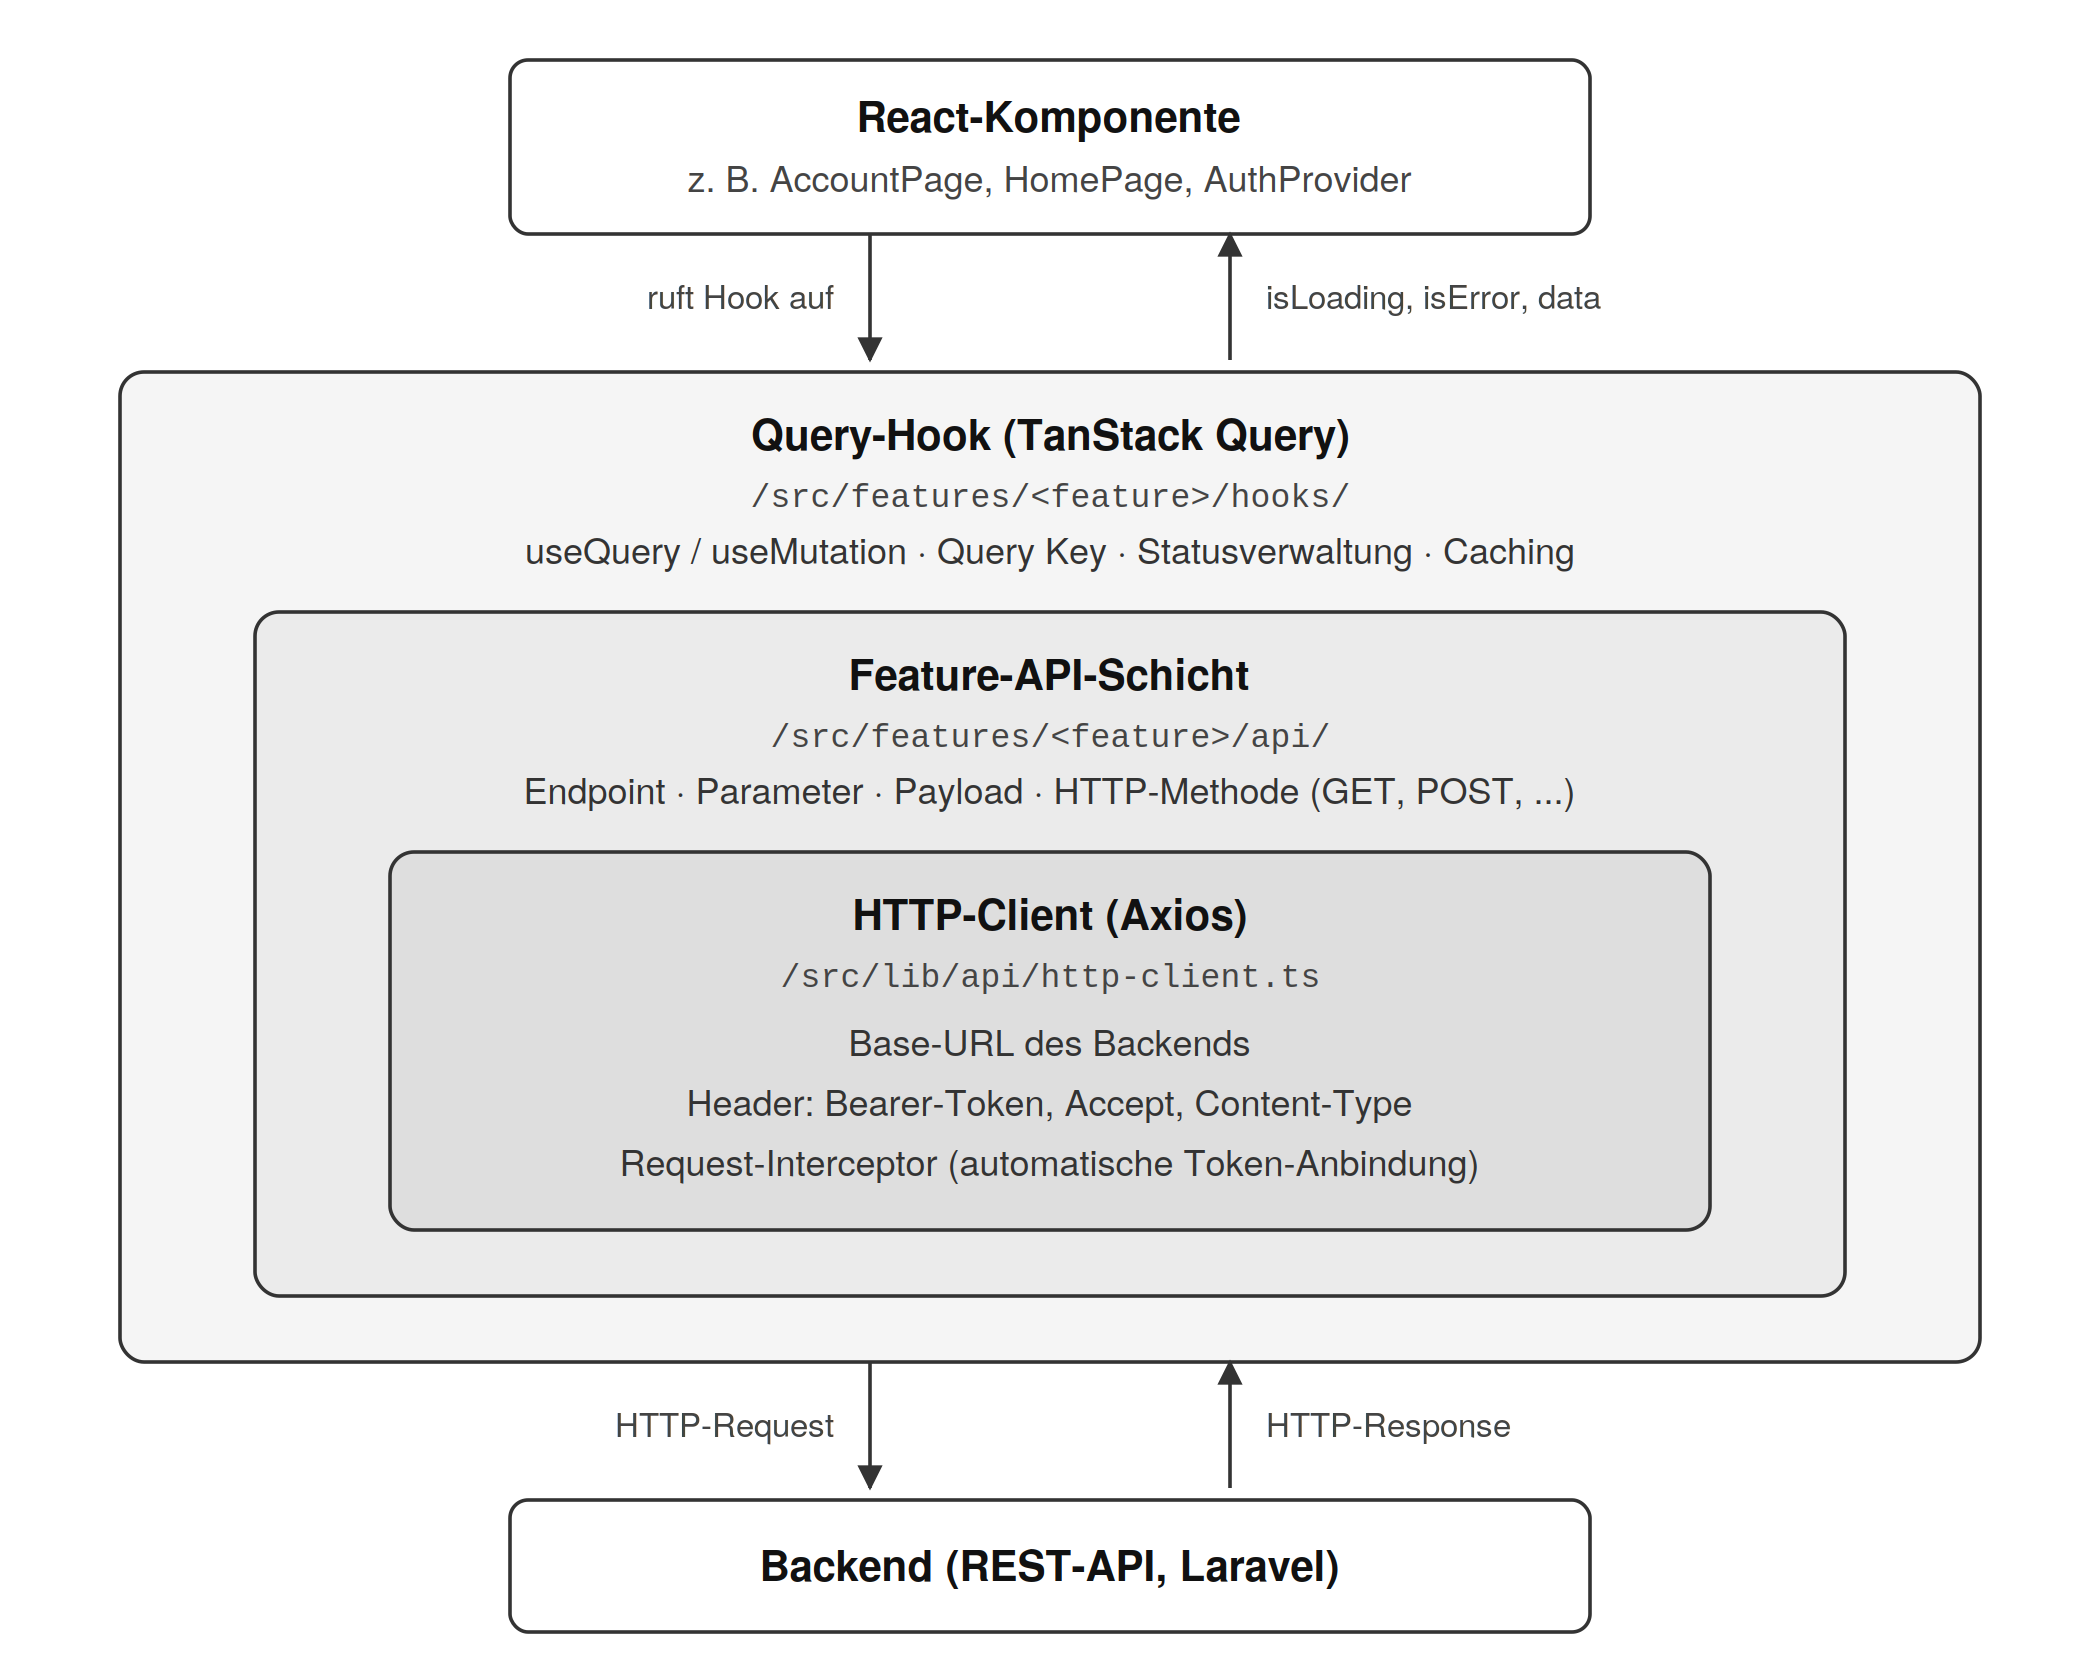
\includegraphics[width=0.75\textwidth]{Bilder/abb_netzwerk_schichten.png}
\caption{Drei-Schichten-Modell der Netzwerkkommunikation im Frontend von Bazario}
\label{fig:netzwerk_schichten}
\end{figure}



Ein wesentliches Ziel dieses Konzepts ist die einheitliche
Kontrolle über den Zustand jeder Verbindung. Jede Anfrage wird
dabei über einen Query Key identifiziert, der sich aus der
Bezeichnung der Anfrage und ihren Parametern zusammensetzt.
Trifft innerhalb eines kurzen Zeitraums dieselbe Anfrage mit
denselben Parametern erneut ein, erkennt TanStack Query, dass die
zugehörigen Daten bereits im Cache vorliegen, und liefert diese
zurück, anstatt den Server erneut zu kontaktieren; ändern sich
die Parameter, entsteht hingegen ein neuer Query Key und damit
eine neue Anfrage an den Server. Auf dieser Grundlage
unterscheidet die Bibliothek zwischen lesenden Anfragen, die
Daten vom Server abrufen, und schreibenden Operationen, die Daten
auf dem Server verändern. Darüber hinaus bietet
die Bibliothek einen Mechanismus zur gezielten Invalidierung
bereits abgerufener Daten; dieser bildet die projektweit
einheitliche Grundlage für die Aktualität zwischengespeicherter
Daten und wird in Kapitel~\ref{chap:umsetzung} anhand konkreter
Beispiele beschrieben.


Das beschriebene Konzept ergänzt das in
Abschnitt~\ref{subsec:state-management-konzept} dargestellte
globale State Management: Entsprechend der in
Abschnitt~\ref{subsec:state-management} eingeführten Trennung
verwaltet Zustand den clientseitigen Anwendungszustand, während
TanStack Query für den serverseitigen Datenbestand zuständig
ist, der über die beschriebenen Schichten abgerufen und
synchronisiert wird.


\section{UI/UX-Konzept}
\label{sec:uiux_konzept}
\subsection{Gestaltungsansatz und Leitlinien}
\label{subsec:gestaltungsansatz}
 
Die Oberfläche von \textit{Bazario} ist nicht als gestalterische
Schicht über der Anwendung entworfen, sondern als Teil ihrer
Struktur. Da die Plattform Produktkauf, Dienstleistungsbuchung,
Zahlung, Nachrichten und Kontoverwaltung in einem System vereint,
muss sie mehrere voneinander unabhängige Arbeitsabläufe tragen, ohne
dass die Bedienung mit jedem hinzukommenden Bereich unübersichtlicher
wird.
 
Maßgeblich für den Entwurf ist deshalb die Funktion einer Ansicht,
nicht ihr Erscheinungsbild. Jede Seite ist um diejenige Handlung
herum aufgebaut, die auf ihr im Vordergrund steht: Produktseiten um
das Sichten eines Angebots, Dienstleistungsseiten um die Wahl eines
Termins, Kontoseiten um die Verwaltung laufender Vorgänge. Das
Bedienmodell bleibt dadurch über die Anwendung hinweg gleich, auch
wenn die zugrunde liegenden Abläufe unterschiedlich komplex sind.
 
Die vier in Abschnitt~\ref{subsec:gestaltungsprinzipien} verdichteten
Anforderungen gelten dabei durchgehend: Konsistenz über gleichartige
Situationen hinweg, Erkennbarkeit des Systemzustands, Vermeidung von
Fehleingaben und Kontrolle des Nutzers über den Ablauf.
 
Hinzu tritt eine fünfte Leitlinie, die sich aus dem Rollenmodell
ergibt und in den allgemeinen Prinzipienkatalogen nicht vorkommt:
Rollensensitivität. Kunde, Verkäufer und Dienstleister rufen dieselbe
Anwendung aus unterschiedlichen Gründen auf. Einen Kunden beschäftigen
Katalog, Bestellung und Buchung; einen Verkäufer seine Produkte, die
eingegangenen Bestellungen und die Einnahmen; einen Dienstleister
zusätzlich Verfügbarkeit und Terminanfragen. Die Oberfläche gewichtet
daher je nach zugewiesener Rolle anders, ohne das gemeinsame
gestalterische System zu verlassen: Es ändert sich, was zuerst
erscheint, nicht wie es aussieht (vgl.
Abschnitt~\ref{subsec:verkaeufer_dashboard_konzept}).
 
Aus diesem Ansatz folgen vier Vorgaben, die den in den nächsten
Abschnitten beschriebenen Entscheidungen zugrunde liegen:
 
\begin{itemize}
\item Wiederkehrende Muster -- Karten, Schaltflächen, Dialoge,
      Zustandsmarkierungen, Formularabschnitte -- folgen denselben
      Regeln, statt je Ansicht neu festgelegt zu werden.
\item Der jeweils nächste sinnvolle Schritt einer Seite ist
      hervorgehoben; ergänzende Angaben treten zurück.
\item Farbe trägt Bedeutung und wird nicht zur Verzierung eingesetzt.
\item Eine nicht verfügbare Handlung wird benannt und begründet,
      statt stillschweigend zu entfallen.
\end{itemize}
 
Die letzte Vorgabe wiegt schwerer, als sie zunächst wirkt: Sie
betrifft die Fristen für Stornierung und Verlegung ebenso wie nicht
belegbare Tage in der Terminauswahl und ist an beiden Stellen
unabhängig voneinander angewandt worden (vgl.
Abschnitt~\ref{subsec:verkaeufer_dashboard_konzept} und
Abschnitt~\ref{subsec:buchung_konzept}).
 
Ergänzend gilt ein Grundsatz der Beschränkung: Bestandteile, die
lediglich vorhandene Wege wiederholen, entfallen. Eine Fußzeile
etwa nähme üblicherweise Angaben zum Betreiber, Verweise auf soziale
Netzwerke und Schnellzugriffe auf -- Inhalte, die entweder bereits in
der Kopfzeile erreichbar sind oder für den Funktionsumfang der
Plattform keine Rolle spielen. Verzichtet wird damit nicht auf
Gestaltung, sondern auf Doppelung.

\subsection{Designsystem und Farbschema}
\label{subsec:designsystem}
Das Designsystem von \textit{Bazario} setzt das in
Abschnitt~\ref{subsec:designsysteme} beschriebene Prinzip um, die
visuellen Grundelemente einer Anwendung nicht in den Komponenten zu
verstreuen, sondern als benannte Werte an einer Stelle zu pflegen.
Umgesetzt ist dies über \acs{CSS}-Variablen, die in der globalen
Stildatei definiert und über die Tailwind-Konfiguration als
Utility-Klassen verfügbar gemacht werden (vgl.
Abschnitt~\ref{subsec:ui-bibliotheken}).
 
Die Farbwerte sind nicht als Einzelfarben benannt, sondern nach ihrer
Funktion in der Oberfläche. Jede Fläche besitzt einen zugehörigen
Vordergrundwert, etwa \texttt{background} mit \texttt{foreground},
\texttt{card} mit \texttt{card-foreground} oder \texttt{primary} mit
\texttt{primary-foreground}. Diese paarweise Definition stellt sicher,
dass Text und Hintergrund nicht unabhängig voneinander geändert
werden können und ein Kontrastverhältnis damit nicht versehentlich
verloren geht. Ergänzt wird das Schema um Tokens für Rahmen,
Eingabefelder und Fokusringe sowie um einen eigenen Wert
\texttt{destructive} für zerstörende Aktionen und Fehlerzustände.
 
Als Farbraum wird durchgängig \acs{OKLCH} verwendet. Anders als bei
hexadezimalen Angaben entspricht die Helligkeitskomponente dort
näherungsweise der wahrgenommenen Helligkeit, wodurch sich
Farbabstufungen gleichmäßig ableiten lassen \cite{css_color_4}. Die
Palette ist bewusst neutral gehalten: Sämtliche Flächen- und
Textfarben besitzen keinen Buntanteil, allein \texttt{destructive}
ist als roter Farbwert angelegt. Farbe wird damit ausschließlich dort
eingesetzt, wo sie eine Bedeutung trägt, während die inhaltliche
Gliederung über Helligkeit, Abstände und Typografie erfolgt.
 
Diese Zurückhaltung erklärt eine Entscheidung, die auf den ersten
Blick überrascht: Karten tragen dieselbe Flächenfarbe wie die Seite,
auf der sie liegen. Ihre Abgrenzung entsteht allein über den Rahmen.
Eine zweite Flächenfarbe hätte die Palette erweitert und müsste mit
sämtlichen darauf erscheinenden Texten und Schaltflächen abgestimmt
werden; der Rahmen leistet dieselbe Trennung, ohne einen weiteren
Farbwert einzuführen. Er ist deshalb bewusst nahe am Hintergrund
gewählt -- deutlich genug, um zu trennen, zurückhaltend genug, um
nicht mit dem Inhalt zu konkurrieren.
 
Der Wert \texttt{primary} kennzeichnet die jeweils vorrangige
Handlung einer Ansicht, also diejenige, die weitere Vorgänge erst
ermöglicht: die Anmeldung, das Auslösen des Checkouts, die Übernahme
einer Buchung in den Warenkorb. Handlungen ohne diese Wirkung
erhalten die zurückhaltendere Darstellung über \texttt{secondary} --
die Abmeldung etwa ist keine vorrangige Handlung und wird deshalb
anders dargestellt als die Anmeldung an derselben Stelle.
\texttt{muted} kennzeichnet Elemente ohne gegenwärtige Wirkung, also
insbesondere deaktivierte Schaltflächen.
 
Ein zweites vollständiges Token-Set ist für die dunkle Darstellung
hinterlegt und wird über eine Variante am Wurzelelement aktiviert.
Da die Komponenten ausschließlich die funktionalen Token
referenzieren und keine festen Farbwerte enthalten, erfordert der
Wechsel keine Änderung an den Komponenten selbst.
 
Die Eckenradien folgen demselben Prinzip. Definiert ist ein einziger
Basiswert von 0,625\,rem; die Abstufungen von klein bis sehr groß
ergeben sich daraus über feste Zuschläge in Schritten von vier
Pixeln. Dass überhaupt mehrere Stufen nötig sind, liegt an der
Wahrnehmung: Derselbe Radius wirkt an einer bildschirmbreiten Fläche
kaum, an einer kleinen Schaltfläche dagegen stark. Elemente
vergleichbarer Größe erhalten deshalb denselben Wert, größere und
kleinere jeweils eine benachbarte Stufe.
 
Für die Typografie wird mit \textit{Geist} eine variable Schriftart
eingebunden und über die Tokens für Fließtext und Überschriften
referenziert. Die Größen folgen einer Staffel: Seitentitel benennen
die aufgerufene Ansicht, Abschnittstitel gliedern sie, Kartentitel
bezeichnen einzelne Gegenstände wie Bestellungen oder
Dienstleistungen; darunter stehen der Fließtext in einer einzigen
Größe sowie gedämpfte Angaben für Metadaten und Hilfetexte. Die
Unterscheidung erfolgt dabei nicht ausschließlich über die Größe:
Wo zwei Angaben gleich groß erscheinen, etwa eine Feldbeschriftung
und der zugehörige Hinweis, trennt sie die Farbe. Diese Staffelung ist
auf den Konto- und Bestellseiten maßgeblich, wo zahlreiche
gleichrangig wirkende Angaben nebeneinander stehen und ohne
Gliederung schwer zu überblicken wären.
 
Das Farbschema und die Komponentenbasis entsprechen der neutralen
Standardkonfiguration von shadcn/ui \cite{shadcn_docs}. Diese wurde
übernommen, weil sie die in Abschnitt~\ref{subsec:designsysteme}
genannten Anforderungen an Konsistenz bereits erfüllt; eine eigene
Gestaltung der Grundelemente war für den Funktionsumfang dieser
Arbeit nicht erforderlich.
 
Die paarweise Definition von Fläche und Vordergrund erlaubt es, die
Anforderungen aus Abschnitt~\ref{subsec:barrierefreiheit} unmittelbar
am Farbsystem zu prüfen. Für den Fließtext auf heller Fläche ergibt
sich ein Kontrastverhältnis von 19,8:1, für gedämpften Text 4,6:1;
beide erfüllen Erfolgskriterium 1.4.3 der Stufe AA. Für
Bedienelemente und Zustandsanzeigen gilt mit Kriterium 1.4.11 ein
eigener Schwellenwert von 3:1, dessen Prüfung in
Kapitel~\ref{chap:testen} erfolgt.


\subsection{Seitenstruktur und Navigationsprinzip}
\label{subsec:seitenstruktur}
Sämtliche Ansichten der Anwendung sind in einen gemeinsamen Rahmen
eingefasst, der aus der in Abschnitt~\ref{subsec:routing-konzept}
beschriebenen Routenhierarchie folgt: Die Layout-Komponente bildet
die oberste Ebene, alle Seiten werden als deren Kindrouten
dargestellt. Was sich beim Wechsel einer Seite ändert, ist damit
allein der Inhaltsbereich; die Kopfzeile bleibt bestehen.
Abbildung~\ref{fig:rahmen} zeigt diesen Aufbau.
 
\begin{figure}[H]
\centering
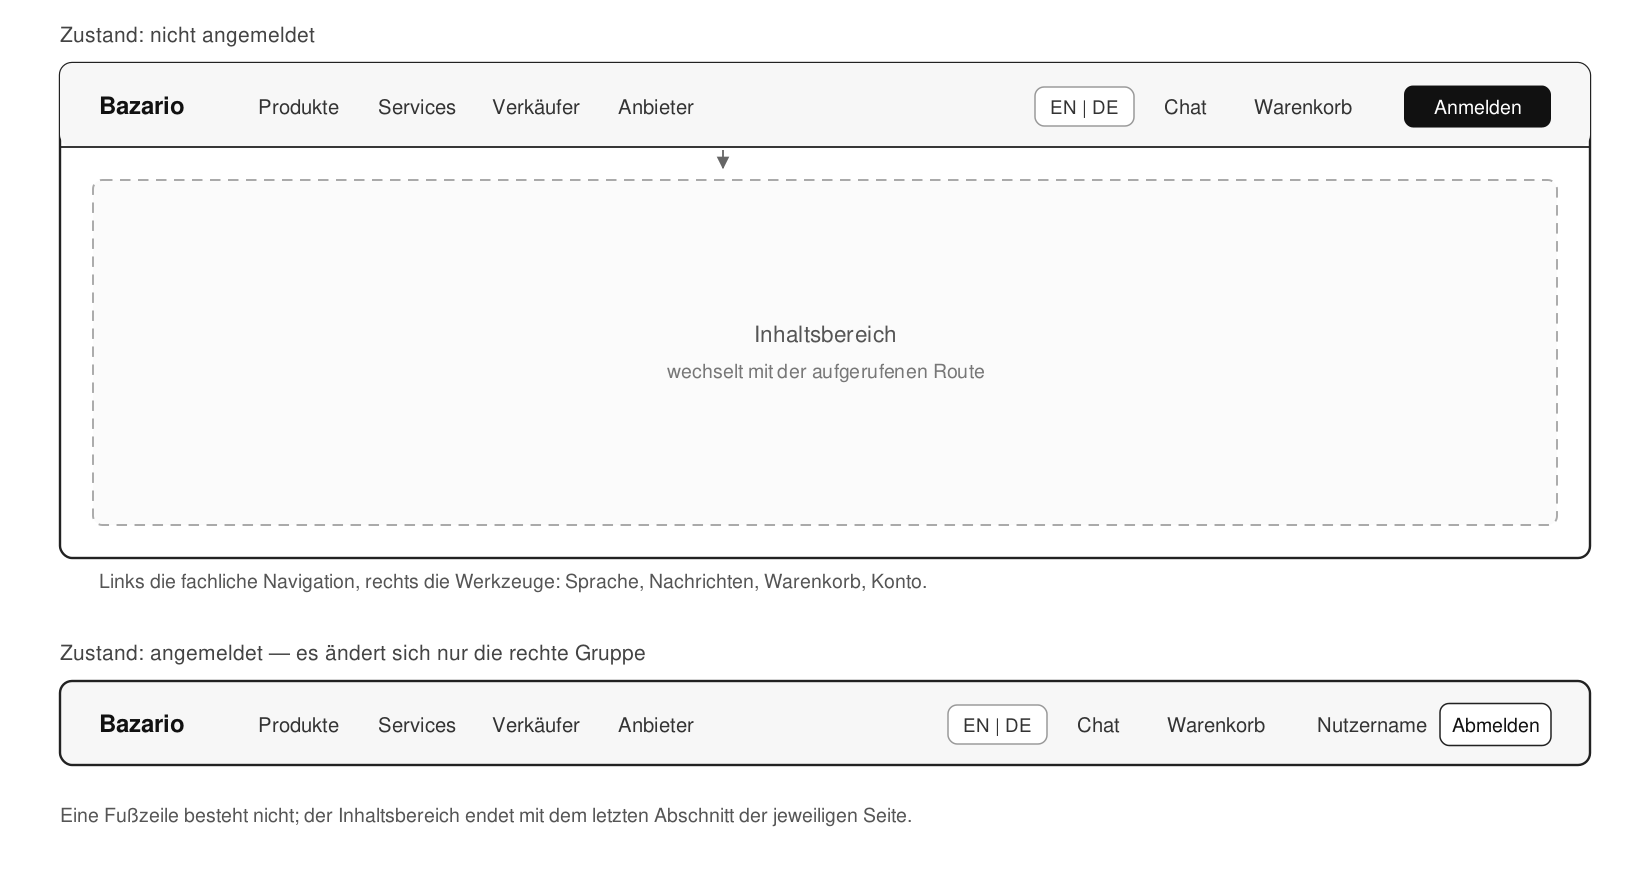
\includegraphics[width=0.80\textwidth]{Bilder/abb_rahmen.png}
\caption{Aufbau des Anwendungsrahmens in beiden Anmeldezuständen
(Strukturskizze, eigene Darstellung)}
\label{fig:rahmen}
\end{figure}
 
Die Kopfzeile ist in zwei Gruppen geteilt. Links steht neben dem
Namen der Plattform die fachliche Navigation mit den vier
öffentlichen Katalogbereichen -- Produkte, Dienstleistungen,
Verkäufer und Anbieter (vgl.
Abschnitt~\ref{subsec:katalog_konzept}). Rechts stehen die
Werkzeuge, die den Nutzer selbst betreffen: die Sprachwahl (vgl.
Abschnitt~\ref{subsec:mehrsprachigkeit_konzept}), der Zugang zu den
Nachrichten (vgl. Abschnitt~\ref{subsec:messaging_konzept}), der
Warenkorb und der Kontobereich.
 
Zwischen den beiden Anmeldezuständen ändert sich nur diese rechte
Gruppe: An die Stelle der Schaltfläche zur Anmeldung treten der Name
des Nutzers und die Abmeldung. Die fachliche Navigation bleibt
unverändert, da die Katalogbereiche allen Nutzern offenstehen. Der
Rahmen erfüllt damit die in
Abschnitt~\ref{subsec:gestaltungsprinzipien} genannte Anforderung
nach Konsistenz über gleichartige Situationen hinweg: Ein Nutzer, der
sich anmeldet, findet dieselbe Oberfläche vor und muss sich nicht neu
orientieren.
 
Eine Fußzeile besteht nicht (vgl.
Abschnitt~\ref{subsec:gestaltungsansatz}); der Inhaltsbereich endet
mit dem letzten Abschnitt der jeweiligen Seite, sodass sämtliche
Navigation an einer einzigen Stelle zusammenläuft.
 
Wie sich eine konkrete Seite in diesen Rahmen einfügt, zeigt
Abbildung~\ref{fig:startseite} am Beispiel der Startseite.
 
\begin{figure}[H]
\centering
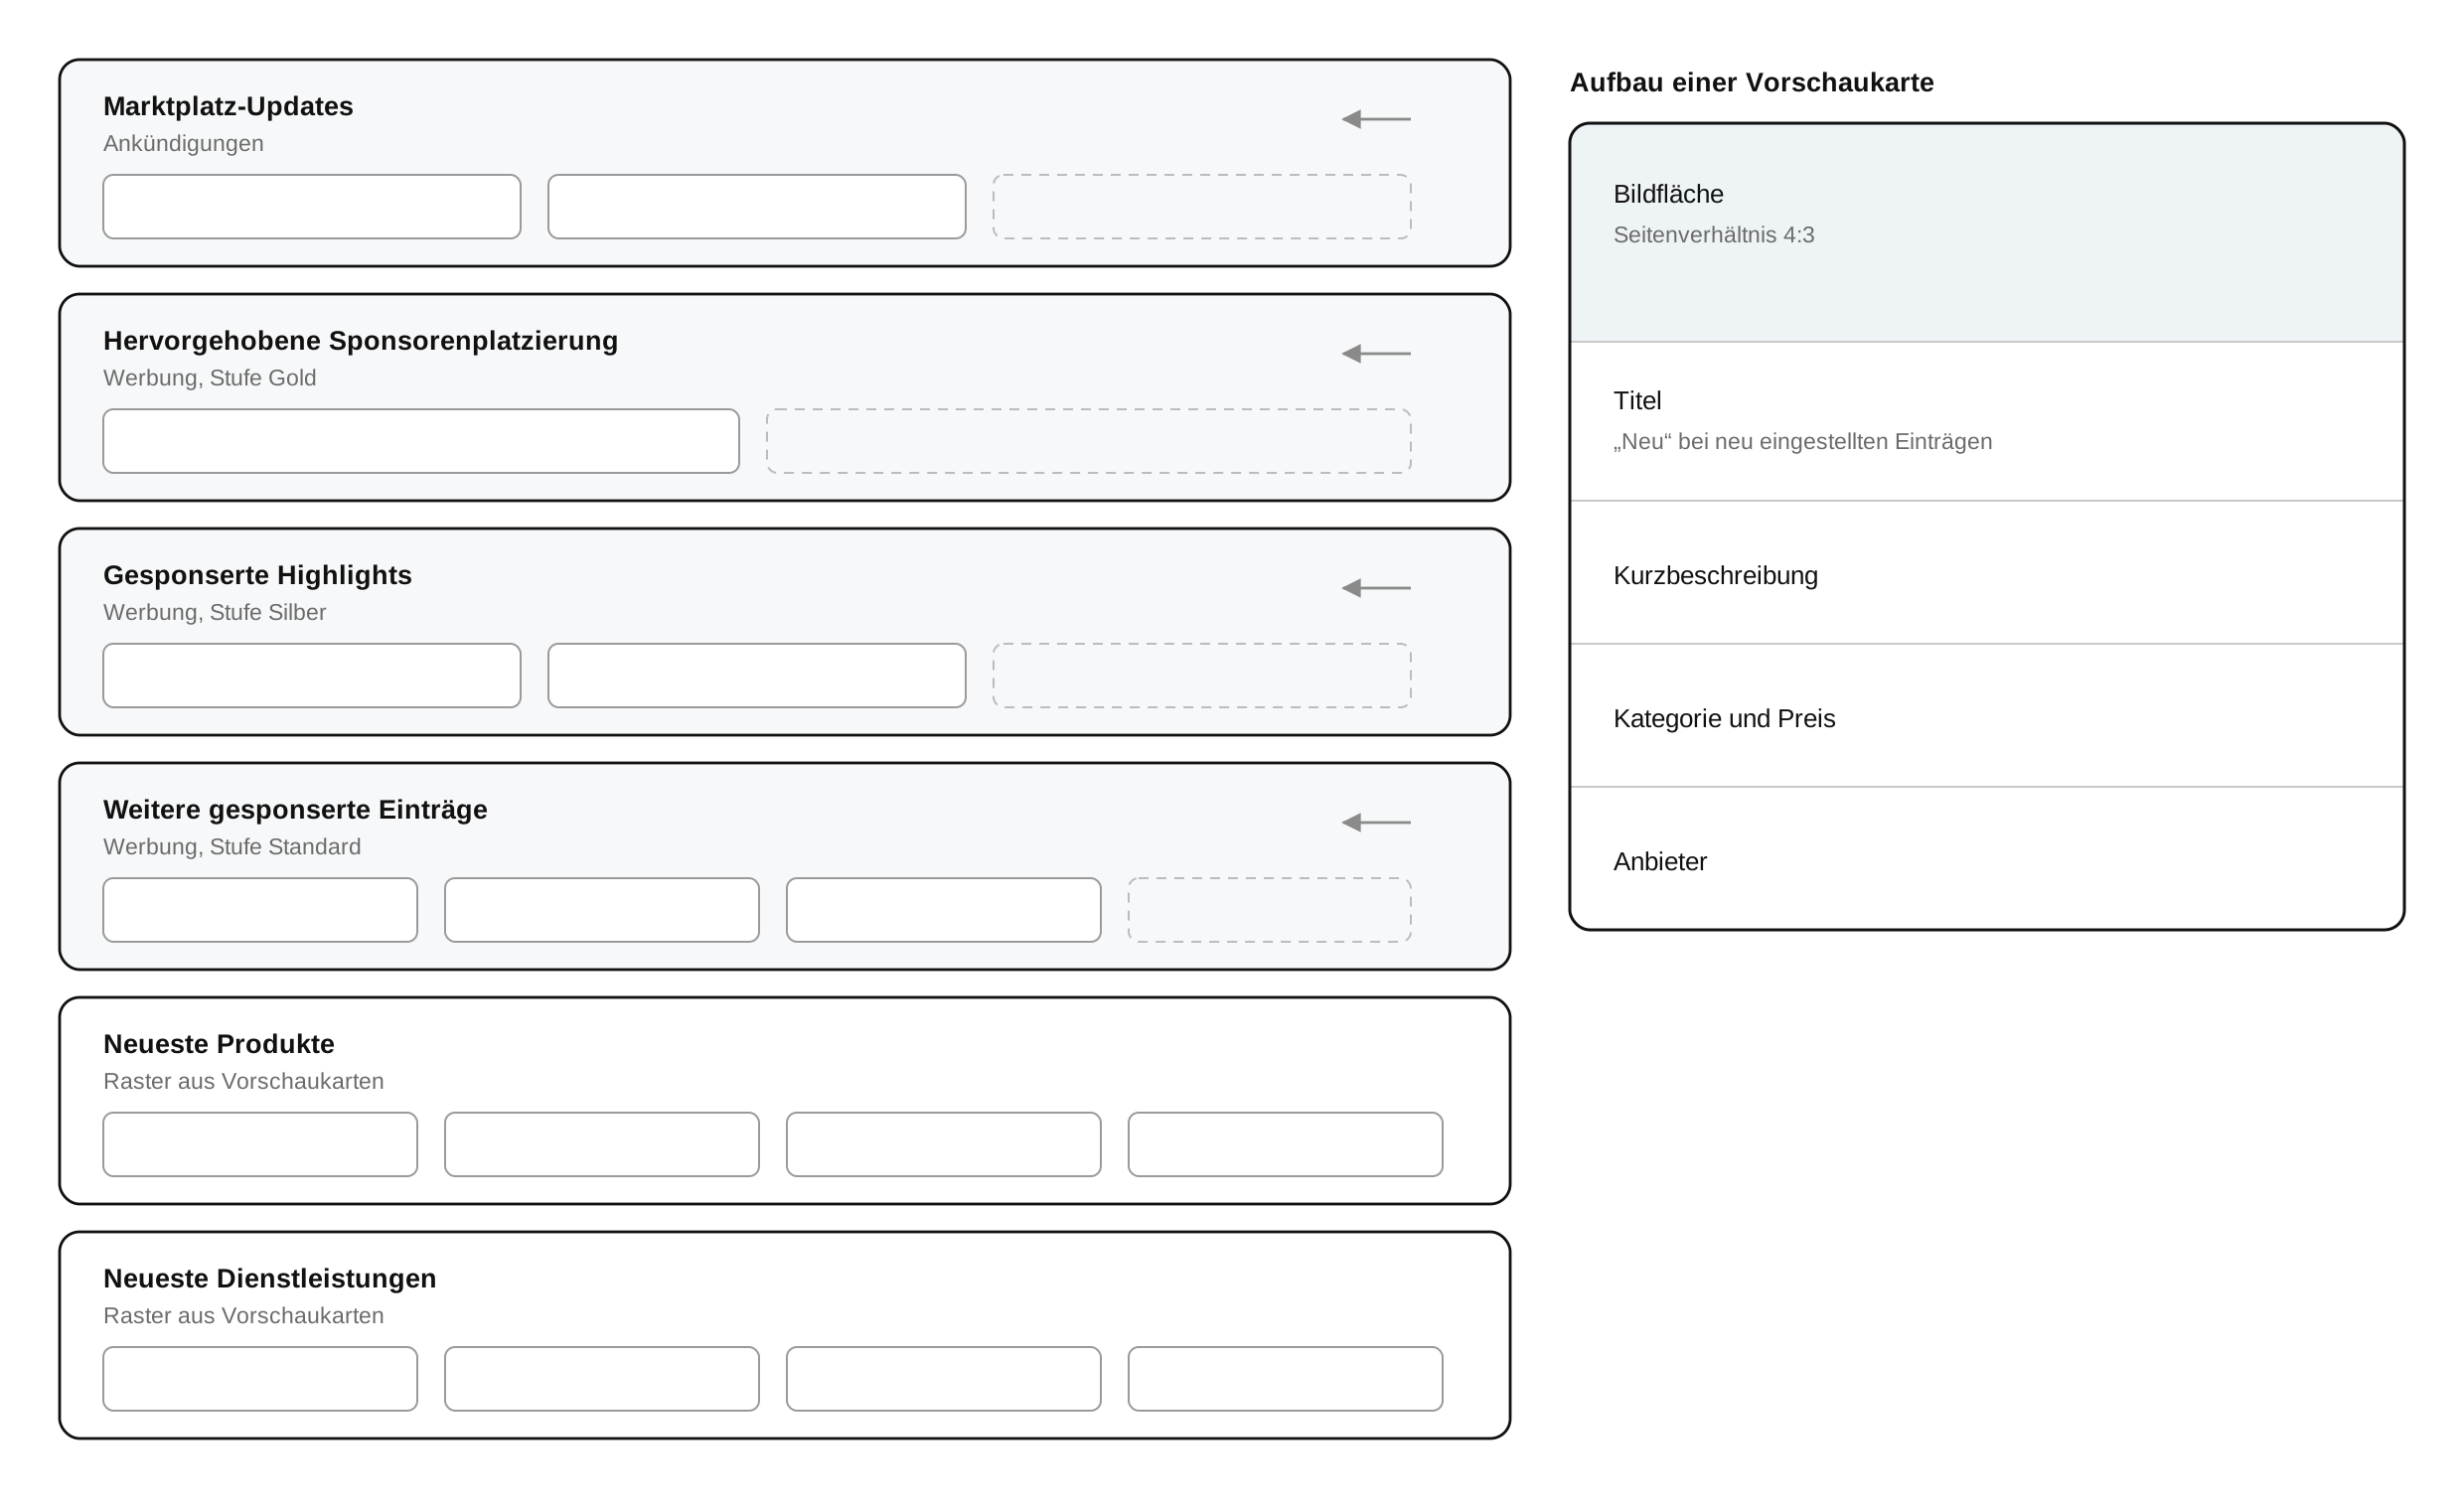
\includegraphics[width=\textwidth]{Bilder/abb_startseite.png}
\caption{Struktur der Startseite und Aufbau einer Vorschaukarte
(Strukturskizze, eigene Darstellung)}
\label{fig:startseite}
\end{figure}
 
Auf den Seitentitel mit einem einleitenden Satz folgen zwei
gleichartig aufgebaute Abschnitte, einer für die zuletzt
eingestellten Produkte und einer für die zuletzt eingestellten
Dienstleistungen. Beide bestehen aus einer Überschrift und einem
Raster aus Vorschaukarten.
 
Die Karte ist dabei das durchgehende Gestaltungselement des
Katalogbereichs. Sie führt von oben nach unten die Bildfläche, den
Titel, eine Kurzbeschreibung, die Kategorie zusammen mit dem Preis
und schließlich den Anbieter. Produkte und Dienstleistungen
verwenden dieselbe Karte in derselben Anordnung; sie unterscheiden
sich allein in der Hintergrundfarbe der Bildfläche. Dieselbe Karte
wird auf den Katalogseiten und den Profilseiten der Anbieter erneut
verwendet, sodass ein Angebot überall in derselben Form erscheint --
die technische Grundlage dafür bildet das in
Abschnitt~\ref{subsec:komponentenarchitektur} beschriebene
Komponentenmodell.
 
Die Zahl der Karten je Zeile richtet sich nach der verfügbaren
Anzeigefläche und verringert sich auf schmalen Bildschirmen, ohne
dass der Aufbau der einzelnen Karte sich ändert. Das entspricht dem
in Abschnitt~\ref{subsec:responsive-design} beschriebenen Vorgehen,
die Anordnung der Elemente an Umbruchpunkten anzupassen, statt eine
zweite Oberfläche vorzuhalten.
 
Auf schmalen Anzeigeflächen ändert sich jedoch nicht nur die
Spaltenzahl. Die Kopfzeile trägt nebeneinander die Navigation, die
Sprachwahl, den Zugang zu Nachrichten und Warenkorb sowie den
Kontobereich; auf geringer Breite würde diese Reihe umbrechen und die
Bedienung erschweren. Sie wird deshalb unterhalb eines Umbruchpunkts
zu einem aufklappbaren Menü zusammengefasst, sodass die obere Leiste
kompakt bleibt.
 
Ebenso ändert sich die Reihenfolge innerhalb der Karten. Eine
Anordnung, die auf breiter Fläche übersichtlich wirkt, führt auf
schmaler entweder zu übermäßiger Breite oder zu leeren Bereichen.
Titel, Preis, Zeitangabe und die zugehörige Handlung bleiben deshalb
zuerst sichtbar, während ergänzende Angaben darunter rücken. Die
Terminauswahl ist dabei der empfindlichste Fall: Tageswahl,
Zeitfensterliste, Zeitzone und Zusammenfassung müssen auch auf
geringer Breite zusammenhängend erkennbar bleiben, da eine
unvollständig erfasste Auswahl unmittelbar zu einer falschen Buchung
führen würde.
 
Am Fuß der Seite ist ein Bereich für Werbung und Ankündigungen
vorgesehen; er ist in Abbildung~\ref{fig:startseite} gestrichelt
dargestellt.

\subsection{Barrierefreiheit im Entwurf}
\label{subsec:barrierefreiheit_konzept}
 
Barrierefreiheit ist im Entwurf als Qualitätsanforderung behandelt,
nicht als Nachweisziel. Maßgeblich sind die vier in
Abschnitt~\ref{subsec:barrierefreiheit} genannten Erfolgskriterien;
ihre Prüfung erfolgt in Kapitel~\ref{chap:testen}.
 
Vier Festlegungen ergeben sich daraus für den Entwurf.
 
Erstens werden Bedienelemente ihrer Bedeutung entsprechend gewählt:
Navigation als Verweis, eine auslösende Handlung als Schaltfläche,
eine Rückfrage als Dialogkomponente und nicht als browsereigene
Abfrage. Damit ist die Bedeutung eines Elements nicht nur visuell,
sondern auch im Dokument hinterlegt und für assistive Technologien
zugänglich. Handlungen mit nicht umkehrbarer Wirkung -- das Löschen
einer Dienstleistung, eines Produkts oder des eigenen Kontos --
werden zusätzlich über einen Bestätigungsdialog geführt, sodass der
Nutzer die Kontrolle über den Ablauf behält (vgl.
Abschnitt~\ref{subsec:gestaltungsprinzipien}).
 
Zweitens erhält jedes bedienbare Element einen sichtbaren
Fokuszustand. In Abläufen mit mehreren aufeinanderfolgenden
Bedienschritten -- Anmeldung, Terminauswahl, Kontoverwaltung -- muss
ohne Zeigegerät erkennbar bleiben, welches Element gerade angesteuert
ist.
 
Drittens tragen Eingabefelder eine eigene Beschriftung statt
lediglich eines Platzhaltertextes, und Fehlermeldungen erscheinen an
einer festen Stelle unterhalb des betroffenen Feldes. Ein
Platzhalter verschwindet mit der ersten Eingabe; die Angabe, was das
Feld erwartet, wäre damit genau dann nicht mehr verfügbar, wenn sie
überprüft werden soll.
 
Viertens bleibt eine nicht verfügbare Handlung sichtbar und wird
begründet, statt entfernt zu werden. Diese bereits in
Abschnitt~\ref{subsec:gestaltungsansatz} genannte Vorgabe hat hier
eine zweite Begründung: Ein Bedienelement, das erst nach dem Auslösen
fehlschlägt, teilt den Systemzustand später mit als eines, das seinen
Zustand von vornherein anzeigt.
\subsection{Mehrsprachigkeit und Sprachwahl}
\label{subsec:mehrsprachigkeit_konzept}
 
\textit{Bazario} folgt der in
Abschnitt~\ref{subsec:mehrsprachigkeit} beschriebenen Zweiteilung:
Die Oberflächentexte werden im Frontend übersetzt, die Angaben zu
Produkten, Dienstleistungen und Anbietern liefert das Backend bereits
in der angeforderten Sprache. Diese Aufteilung folgt aus der Herkunft
der Daten, nicht aus einer Entwurfsentscheidung -- ein Anbieter
erfasst Titel und Beschreibung mehrsprachig (vgl.
Abschnitt~\ref{subsec:verkaeufer_dashboard_konzept}), weshalb nur das
Backend beide Fassungen kennt.
 
Die Sprachwahl ist im Anwendungsrahmen angeordnet und damit von jeder
Seite aus erreichbar. Sie wirkt ohne erneutes Laden, da ein Neuladen
den Zustand der Ansicht verwerfen würde, etwa eine begonnene Eingabe.
Beim ersten Aufruf gilt die im Browser eingestellte Sprache, sofern
sie unterstützt wird, andernfalls Englisch; die anschließend
getroffene Wahl wird gespeichert und bei späteren Besuchen
wiederhergestellt.
 
Angeboten werden Deutsch und Englisch, für die Oberflächentexte
vollständig umgesetzt. Bei den Inhalten reicht die Wahl gegenwärtig
nicht so weit: Die Erfassungsformulare sehen Englisch und Arabisch
vor, sodass eine deutsche Fassung nicht entsteht. Anforderung und
Verfügbarkeit einer Sprache sind damit zwei getrennte Fragen -- das
Frontend kann jede Sprache anfordern, geliefert wird nur, was zuvor
erfasst wurde.

% ----------------------------------------------------------------
\section{Konzept der einzelnen Funktionsbereiche}
\subsection{Authentifizierung und Onboarding}
\label{subsec:auth-onboarding}

Der Login erfolgt über einen Dialog, der von
jeder Stelle der Anwendung aus aufgerufen werden
kann, ohne die aktuelle Seite zu verlassen,
sodass ein Nutzer etwa während des Checkouts
nicht unterbrochen wird. Die Registrierung
erfolgt dagegen über eine eigene Seite, da sie
mehr Eingabefelder benötigt und eine
eigenständige Handlung darstellt. Beide
Formulare validieren ihre Eingaben clientseitig,
bevor eine Anfrage gestellt wird; serverseitige
Fehler werden gezielt dem betroffenen Feld
zugeordnet, und der Absende-Button wird während
der Bearbeitung deaktiviert.

Verläuft Anmeldung oder Registrierung
erfolgreich, bildet die Anwendung aus der
Backend-Antwort eine Sitzung mit
Zugriffstoken, Nutzerdaten und Rollen. Diese wird
im localStorage gespeichert, um den Anmeldestatus
über Neuladen und erneute Besuche hinweg zu
erhalten, und reaktiv über Zustand
bereitgestellt (vgl.
Abschnitt~\ref{subsec:state-management-konzept}).
Der Zugriff auf geschützte Bereiche wird über ein
dreistufiges Konzept sichergestellt: Zunächst
wird geprüft, ob der Anmeldestatus bereits
bestimmt ist (Ladezustand), dann ob der Nutzer
angemeldet ist (sonst Weiterleitung), und erst
danach wird der geschützte Inhalt angezeigt.

Der gespeicherte Token wird automatisch über
einen zentralen, wiederverwendbaren Mechanismus
an jede Anfrage angehängt und zusätzlich aktiv
beim Backend validiert, sodass ein abgelaufener
oder ungültiger Token erkannt und der Nutzer
korrekt abgemeldet wird. Für das Onboarding
verfolgt die Plattform ein zweistufiges
Rollenmodell: Jeder Nutzer erhält zunächst die
Rolle \textit{Customer}, ein Wechsel zu \textit{Seller} oder
\textit{ServiceProvider} erfolgt über einen von einem
Administrator geprüften Antragsprozess.
 
 
 
\subsection{Katalog- und Detailseiten}
\label{subsec:katalog_konzept}

Der Katalogbereich von \textit{Bazario}
umfasst die Startseite, die
Katalogseiten für Produkte und
Dienstleistungen sowie die öffentlichen
Profilseiten einzelner Verkäufer und
Dienstleister.

Die Startseite fasst Ankündigungen, Werbeplatzierungen sowie
eine Vorschau der zuletzt hinzugefügten Produkte und
Dienstleistungen in aufeinanderfolgenden Abschnitten zusammen.
Sämtliche Inhalte der Startseite werden über eine einzelne,
gebündelte Anfrage an das Backend abgerufen.

Über eigenständige Katalogseiten
lassen sich alle Produkte
beziehungsweise Dienstleistungen der
Plattform einsehen und nach Kategorie
filtern. Zusätzlich
stellt \textit{Bazario} für jeden
Verkäufer und jeden Dienstleister eine
öffentliche Profilseite bereit, auf
der Kunden ausschließlich die Produkte
beziehungsweise Dienstleistungen
dieses einen Anbieters einsehen
können. Diese öffentlichen
Profilseiten sind von der internen
Verwaltungsseite des jeweiligen
Verkäufers oder Dienstleisters zu
unterscheiden, die in
Abschnitt~\ref{subsec:verkaeufer_dashboard_konzept}
beschrieben wird.

Der Aufruf eines einzelnen Produkts
oder einer einzelnen Dienstleistung,
etwa über eine Vorschau-Karte, führt
jeweils auf eine eigene Detailseite.
Für die Darstellung der Vorschauen auf
Startseite und Katalogseiten wird ein
wiederverwendbares Kartenprinzip
verfolgt, das für Produkte und
Dienstleistungen gleichermaßen zum
Einsatz kommt; liegen für einen
Bereich keine Einträge vor, wird dem
Nutzer anstelle einer leeren Fläche
ein entsprechender Hinweis angezeigt.


\subsection{Dienstleistungsbuchung}
\label{subsec:buchung_konzept}
Eine Dienstleistung wird nicht wie ein Produkt in den Warenkorb
gelegt, sondern zuvor auf einen konkreten Termin festgelegt. Der
Entwurf muss daher eine Auswahl anbieten, die nur solche Zeitpunkte
enthält, an denen die Leistung tatsächlich erbracht werden kann.
 
Welche Zeitpunkte das sind, ergibt sich aus zwei Gruppen von Angaben,
die beide in Abschnitt~\ref{subsec:verkaeufer_dashboard_konzept}
beschrieben sind. Die erste betrifft den Anbieter als Person: sein
wiederkehrendes Wochenschema und seine eingetragenen
Abwesenheitszeiträume. Die zweite betrifft die einzelne
Dienstleistung: ihre Dauer, das Zeitraster, in dem Termine beginnen
dürfen, und die Anzahl der Kunden, die denselben Zeitraum belegen
können. Hinzu kommen die bereits vergebenen Buchungen. Die Menge der
wählbaren Termine ist damit nicht fest hinterlegt, sondern wird für
jeden Tag neu bestimmt.
 
Die Auswahl erfolgt in zwei Schritten: zuerst der Tag, dann das
Zeitfenster. Eine gemeinsame Liste aller Termine über mehrere Wochen
hinweg wäre unübersichtlich, und die Zahl der Einträge stiege mit
einem feineren Zeitraster weiter an. Erst nach der Wahl eines Tages
werden dessen Zeitfenster abgerufen und angezeigt.
 
Zu jedem Zeitfenster wird die verbleibende Kapazität angegeben. Bei
Dienstleistungen, die mehrere Kunden gleichzeitig annehmen können,
ist andernfalls nicht erkennbar, ob eine Buchung noch möglich ist
oder das Fenster lediglich noch nicht ausgebucht wirkt.
 
Sämtliche Zeitangaben beziehen sich auf die Zeitzone des Anbieters,
die zusammen mit dem Termin angezeigt wird. Da Anbieter und Kunde in
verschiedenen Zeitzonen ansässig sein können, wäre eine Angabe ohne
Bezugspunkt mehrdeutig; die Zeitzone des aufrufenden Endgeräts als
Grundlage zu verwenden, würde die Angaben je nach Standort des Kunden
verschieben.
 
Die abgeschlossene Auswahl führt nicht unmittelbar zu einer Buchung,
sondern in den Warenkorb. Damit lassen sich Dienstleistungen und
Produkte in einem gemeinsamen Vorgang bezahlen (vgl.
Abschnitt~\ref{subsec:warenkorb_konzept}), und eine verbindliche
Buchung entsteht erst mit der Zahlung. Solange der Vorgang nicht
abgeschlossen ist, bleibt das Zeitfenster für andere Kunden verfügbar.

\subsection{Warenkorb, Checkout und Zahlung}
\label{subsec:warenkorb_konzept}

Der Warenkorb bildet Produkte und Dienstleistungsbuchungen in
einem gemeinsamen Modell ab, das für beide Positionstypen eine
gemeinsame Basis aus Titel, Bild, Preis und Kategorie sowie
typspezifische Zusatzdaten vorsieht; eine Dienstleistungsbuchung
enthält zusätzlich Beginn, Ende, Zeitzone und Ort der
Leistungserbringung. Der Warenkorb bleibt über einen erneuten
Aufruf der Anwendung hinweg erhalten, sodass bereits
hinzugefügte Positionen auch nach einem Neuladen der Seite
bestehen bleiben. Wird ein bereits enthaltenes Produkt erneut
hinzugefügt, erhöht sich lediglich dessen Menge; eine identische
Dienstleistungsbuchung kann dagegen nicht doppelt hinzugefügt
werden. Die Warenkorbseite gliedert sich in eine Übersicht der
enthaltenen Positionen, getrennt nach Produkten und
Dienstleistungen, sowie eine Zusammenfassung mit Anzahl je
Positionstyp und Zwischensumme.

Der Checkout setzt eine angemeldete Sitzung voraus. Ist der Nutzer
nicht angemeldet, öffnet sich der in
Abschnitt~\ref{subsec:auth-onboarding} beschriebene Anmeldedialog,
bevor der Vorgang fortgesetzt wird. Die Plattform muss den Vorgang
einem Nutzer zuordnen können, um ihn nachverfolgbar zu machen, dem
Anbieter mitzuteilen, wer bestellt hat, und dem Kunden die Einsicht in
seine Bestellungen zu ermöglichen.
 
Ein Auftrag entsteht bereits vor der Zahlung. Mit dem Auslösen des
Checkouts legt das Backend einen Auftrag mit dem Status
\textit{requires payment} an, ergänzt ihn um die Positionen des
Warenkorbs und fordert anschließend eine Zahlungssitzung an. Bricht
der Nutzer die Zahlung ab, bleibt der Auftrag unbezahlt bestehen und
kann später über die Bestellübersicht abgeschlossen werden. Der
Warenkorb bleibt in diesem Fall unverändert erhalten, damit ein
abgebrochener Vorgang nicht zum Verlust der bereits
zusammengestellten Positionen führt.
 
Von den in Abschnitt~\ref{subsec:online-zahlung} beschriebenen
Einbindungsvarianten nutzt \textit{Bazario} die gehostete
Zahlungsseite (vgl. Abschnitt~\ref{sec:technologieauswahl}). Das
Frontend gestaltet damit keine eigenen Zahlungsformulare, und
sensible Kartendaten erreichen die Plattform zu keinem Zeitpunkt.

Darin liegt zugleich die Begründung für die
eingangs genannte Anmeldepflicht: Plattformen, die einen Kauf ohne
Anmeldung zulassen, wickeln die Zahlung selbst ab und erhalten dabei
zwangsläufig die Daten des Kunden. Bei \textit{Bazario} gehen diese
Daten ausschließlich an den Zahlungsdienst; ohne Anmeldung läge der
Plattform daher keinerlei Information über den Vorgang vor.
 
Dieser Weg hat eine Konsequenz für den Entwurf: Sobald der Nutzer zur Zahlung auf die Seite des Zahlungsdienstes wechselt, verliert die Plattform die unmittelbare Sicht auf den Vorgang. Sie erfährt weder, ob gezahlt wurde, noch von wem. Genau deshalb wird der Auftrag vorab im Backend angelegt und der Zahlungsstatus im Anschluss beim Zahlungsdienst abgefragt \cite{stripe_checkout_docs}.
 
Die Kommunikation mit dem Zahlungsdienst erfolgt ausschließlich über
das Backend, nicht aus dem Browser heraus. Der Grund liegt in der
Authentifizierung gegenüber dem Dienst: Das Eröffnen einer
Zahlungssitzung erfordert einen geheimen Schlüssel, der dem
Plattformbetreiber zugeordnet ist und nicht im Browser des Nutzers
liegen darf. Hinzu kommt, dass die Plattform eine Vielzahl von Nutzern
bedient und die Eröffnung von Zahlungssitzungen kontrolliert erfolgen
muss.
 
Für die Rückleitung nach abgeschlossener oder abgebrochener Zahlung
stellt das Frontend zwei eigene Seiten bereit. Ihre Adressen werden dem
Zahlungsdienst über das Backend mitgeteilt, sodass der Nutzer nach dem
Verlassen der Zahlungsseite auf die passende Seite der Anwendung
zurückgeführt wird. Beide Seiten sind an eine gültige Sitzung
gebunden, da der Ausgang einer Zahlung einem bestimmten Nutzer
zugeordnet ist.
 
Damit Anbieter Zahlungen empfangen können, nutzt \textit{Bazario} das
Konzept verbundener Konten. Die Plattform unterhält ein eigenes Konto
beim Zahlungsdienst; jedem Verkäufer und jedem Dienstleister wird
darunter ein Unterkonto zugeordnet. Dieses Unterkonto wird aus der
Anwendung heraus angelegt, sodass der Anbieter kein eigenes Konto
einrichten und verknüpfen muss. Auf dieser Grundlage lässt sich der
Zahlungsbetrag automatisiert aufteilen: Ein Anteil verbleibt als
Provision bei der Plattform, der übrige Betrag wird dem Anbieter
gutgeschrieben (vgl. Abschnitt~\ref{subsec:marktplatztypen}).
 
Voraussetzung für eine Gutschrift ist ein vollständig eingerichtetes
Unterkonto einschließlich Identitätsprüfung. Solange diese Prüfung
nicht abgeschlossen ist, weist die Anwendung den Anbieter darauf hin
und zeigt weder Guthaben noch Transaktionen an. Die Einnahmenübersicht
stellt anschließend den Verbindungsstatus, das verfügbare Guthaben und
die noch ausstehenden Beträge dar. Die Auszahlung selbst wird über das
Administrationsdashboard des Backends ausgelöst und ist damit nicht
Gegenstand dieser Arbeit (vgl. Abschnitt~\ref{sec:abgrenzung}).


\subsection{Kontobereich und rollenspezifische Funktionen}
\label{subsec:verkaeufer_dashboard_konzept}

Die Kontoseite bildet den zentralen Einstiegspunkt für alle
angemeldeten Nutzer. Sie ergänzt die in
Abschnitt~\ref{subsec:auth-onboarding} beschriebenen Angaben zur
Sitzung um den Überblick über laufende Vorgänge und den Zugang zu den
rollenspezifischen Funktionen. Dafür gliedert sie sich in zwei
Spalten: links der Stand der eigenen Vorgänge, rechts die verfügbaren
Werkzeuge.
 
Die rechte Spalte ist dabei nach Rollen gegliedert, nicht nach
Funktionen. Jede zugewiesene Rolle erhält einen eigenen
Arbeitsbereich. Die Reihenfolge folgt der Häufigkeit des Zugriffs:
Die rollenspezifischen Arbeitsbereiche stehen oben, da sie der Grund
sind, aus dem ein Anbieter die Seite aufruft; der Kundenbereich, den
jeder Nutzer nach dem Rollenmodell aus
Abschnitt~\ref{sec:rollenmodell} ebenfalls besitzt, folgt darunter.
Im Folgenden wird er dennoch zuerst beschrieben, da er die
gemeinsame Grundlage aller Rollen bildet.
 
Zu jedem Eintrag der linken Spalte wird der aktuelle Zustand
angezeigt, bei Buchungen der Bearbeitungsstand, bei Bestellungen der
Zahlungsstatus und beim Zahlungsdienst der Verbindungszustand, und
daneben genau die Aktion, die in diesem Zustand möglich ist, etwa das
Bestätigen einer angefragten Buchung oder das Nachholen einer offenen
Zahlung. Der Systemzustand ist damit erkennbar, ohne dass eine
Detailansicht geöffnet werden muss (vgl.
Abschnitt~\ref{subsec:gestaltungsprinzipien}).
 
 
% --------------------------- KUNDE -------------------------------
 
Der Kundenbereich führt zur eigenen Bestellhistorie und zur
Verfolgung eigener Buchungen. Beide Ansichten werden getrennt
geführt, weil sich Bestellungen und Buchungen in ihrem Zustandsumfang
deutlich unterscheiden: Ein Produkt wird bestellt, bezahlt und
geliefert, während eine Buchung zusätzlich einen Termin, eine
Zeitzone und die Möglichkeit zur Stornierung oder Verlegung besitzt.
 
Die Bestellübersicht führt sämtliche Aufträge des Nutzers mit
Zahlungsstatus, Datum, Gesamtbetrag und Anzahl der Positionen auf. Da
ein Auftrag bereits vor der Zahlung entsteht (vgl.
Abschnitt~\ref{subsec:warenkorb_konzept}), erscheinen dort auch
unbezahlte Aufträge. Für diese bietet die Übersicht zwei Wege an: die
Zahlung nachzuholen oder den Auftrag zu verwerfen. Ohne diese beiden
Möglichkeiten bliebe ein abgebrochener Zahlungsvorgang als Eintrag
bestehen, den der Nutzer weder abschließen noch entfernen könnte. Die
Detailansicht eines Auftrags zeigt darüber hinaus die einzelnen
Positionen und ihren jeweiligen Zustand.
 
Die Buchungsübersicht führt die gebuchten Termine mit
Bearbeitungsstand, Zeitpunkt und Ort. Zu jeder Buchung werden die
beim Anlegen der Dienstleistung festgelegten Fristen als
Buchungsbedingungen angezeigt, getrennt nach Stornierung und
Verlegung. Der Nutzer erfährt damit bereits vor einer Handlung, bis
wann sie möglich ist, und nicht erst beim Versuch. Nach Ablauf einer
Frist wird die zugehörige Schaltfläche deaktiviert und um eine
Erläuterung ergänzt, die den Grund und das Datum des Fristablaufs
benennt. Die Alternative, sie auszublenden, wurde verworfen: Ein
Nutzer, der eine erwartete Funktion nicht vorfindet, sucht sie
zunächst und erfährt nicht, warum sie fehlt. Die Frist markiert dabei nicht nur das Ende einer Bedienmöglichkeit, sondern den Übergang des wirtschaftlichen Risikos: Nach ihrem Ablauf steht der Betrag dem Anbieter zu, unabhängig davon, ob der Kunde die Leistung in Anspruch nimmt. Der Anbieter kennzeichnet die Buchung in
beiden Fällen nach dem Termin als abgeschlossen.
 
Eine Stornierung löst über das Backend eine Rückerstattung aus, deren
Stand in der Buchung nachvollziehbar bleibt. Eine Verlegung verändert
dagegen ausschließlich den Termin; der bezahlte Betrag bleibt
unberührt, weshalb hierfür ein eigener Auswahlschritt vorgesehen ist,
der die verfügbaren Zeitfenster des Anbieters anzeigt. Diese
Möglichkeiten bestehen ausschließlich für Dienstleistungen. Eine
bezahlte Produktbestellung lässt sich nicht mehr rückgängig machen,
da ihr keine terminierte Leistung zugrunde liegt, deren Absage einen
Zeitraum wieder freigäbe.
 
 
% ------------------------ DIENSTLEISTER --------------------------
 
Besitzt ein Nutzer zusätzlich die Rolle des Dienstleisters, tritt ein
Anbieterbereich hinzu. Er führt zur Verwaltung von Dienstleistungen
und Verfügbarkeiten, zu den eingegangenen Buchungen sowie zur
Anbindung an den Zahlungsdienst und zur Einnahmenübersicht (vgl.
Abschnitt~\ref{subsec:warenkorb_konzept}).
 
Die linke Spalte trennt entsprechend die Vorgänge, die andere Nutzer
beim Anbieter ausgelöst haben, von dessen eigenen Bestellungen;
andernfalls würden in einer Liste Vorgänge nebeneinander angezeigt
werden, bei denen der Nutzer einmal Anbieter und einmal Kunde ist.
Beide Listen zeigen nur die neuesten Einträge und verweisen für den
vollständigen Bestand auf eine eigene Seite.
Die eingegangenen Buchungen werden in einer eigenen Ansicht geführt,
da sie im Gegensatz zu Produktbestellungen eine Handlung des
Anbieters erfordern. Eine Buchung durchläuft dabei mehrere Zustände:
Sie erreicht den Anbieter zunächst als Anfrage, wird von ihm
bestätigt und nach erbrachter Leistung als abgeschlossen
gekennzeichnet.
 
Dass eine Buchung trotz bereits erfolgter Zahlung zunächst nur
angefragt ist, ist beabsichtigt. Die Zahlung sichert den Vorgang
finanziell ab, die Zusage über die Leistung selbst gibt jedoch der
Anbieter. Erst mit seiner Bestätigung gilt der Termin als
verbindlich.
 
Zu jeder Buchung werden daher Kunde, Zeitraum und Zeitzone angezeigt
sowie genau die Aktion, die im jeweiligen Zustand möglich ist: Eine
angefragte Buchung lässt sich bestätigen, eine bestätigte nach
erbrachter Leistung abschließen. Der Anbieter muss den Zustand einer
Buchung damit nicht aus dem Zusammenhang erschließen, sondern findet
an jedem Eintrag den nächsten möglichen Schritt (vgl.
Abschnitt~\ref{subsec:gestaltungsprinzipien}).
Der Abschluss ist dabei bewusst nicht an das Ende des Termins gebunden. In der Regel erfolgt er danach, doch teilt ein Kunde vorher mit, dass er die Leistung nicht in Anspruch nehmen wird, kann der Anbieter die Buchung bereits zuvor abschließen. Eine zeitliche Sperre hätte diesen Fall ausgeschlossen, ohne einen Fehler zu verhindern.
 
Dienstleister verwalten ihre Verfügbarkeit über feste
Arbeitszeiten sowie einzelne Abwesenheitszeiträume. Für jeden
Abwesenheitszeitraum werden Beginn und Ende sowie optional ein
Grund erfasst; zusätzlich lässt sich kennzeichnen, ob es sich um
einen offiziellen Feiertag oder eine persönliche Abwesenheit
handelt, damit Kunden bei der Buchung den Unterschied
nachvollziehen können. Da Dienstleister in unterschiedlichen
Zeitzonen tätig sein können, wird die Zeitzone des jeweiligen
Anbieters bei der Darstellung der Abwesenheitszeiten
berücksichtigt, sodass Zeitangaben nicht in der Zeitzone des
Endgeräts, sondern in der des Anbieters angezeigt werden.
Zusätzlich zu den einzelnen Abwesenheitszeiträumen legen
Dienstleister ein wiederkehrendes Wochenschema mit mehreren
Zeitfenstern je Wochentag fest, das die grundsätzliche
Erreichbarkeit unabhängig von einzelnen Abwesenheiten definiert.
 
Ihre einzelnen Dienstleistungsangebote verwalten Dienstleister
über eine Kartenübersicht, die für jede Dienstleistung Kategorie,
Preis, Dauer und Status anzeigt und das Anlegen, Bearbeiten und
Löschen einzelner Einträge ermöglicht. Titel und Beschreibung
einer Dienstleistung werden dabei jeweils auf Englisch und
Arabisch erfasst, und es lassen sich bis zu fünf Bilder je
Dienstleistung hochladen. Neben diesen Basisdaten legt ein
Dienstleister beim Anlegen oder Bearbeiten einer Dienstleistung
zusätzlich die Regeln für deren spätere Buchung fest: das
Zeitraster, in dem einzelne Termine gebucht werden können, die
maximale Anzahl gleichzeitiger Buchungen, den Ort der
Leistungserbringung sowie getrennte Fristen und Regelungen für
die Stornierung und die Änderung einer bereits bestätigten
Buchung durch den Kunden.
 
 
% -------------------------- VERKÄUFER ----------------------------
 
Für die Rolle des Verkäufers gilt dasselbe Prinzip. Auch hier tritt
ein eigener Arbeitsbereich hinzu, der zur Produktverwaltung sowie zu
Zahlungsdienst und Einnahmenübersicht führt, und auch hier erscheinen
die eingegangenen Bestellungen getrennt von den eigenen.
 
Verkäufer verwalten ihre Produkte über eine analoge
Kartenübersicht, die für jedes Produkt Kategorie und Preis
anzeigt und ebenfalls das Anlegen, Bearbeiten und Löschen
einzelner Einträge ermöglicht. Titel und Beschreibung werden
auch hier auf Englisch und Arabisch erfasst, mit bis zu fünf
Bildern je Produkt. Im Unterschied zu Dienstleistungen entfallen
dabei jedoch die Buchungsregeln.
 
 
% ------------------------ BEIDE ROLLEN ---------------------------
 
Besitzt ein Nutzer beide anbietenden Rollen, erscheinen deren
Arbeitsbereiche untereinander, jeweils zusätzlich zum Kundenbereich.
Nicht zugewiesene Rollen erzeugen dagegen keinen Arbeitsbereich,
sodass die Oberfläche ausschließlich die tatsächlich verfügbaren
Funktionen zeigt. Damit wird die in Abschnitt~\ref{subsec:rbac}
beschriebene rollenbasierte Zugriffskontrolle auf der Ebene der
Benutzerführung umgesetzt.
 
Unterhalb der Arbeitsbereiche folgen die rollenunabhängigen
Funktionen: Passwortänderung, Rollenwechselantrag und Kontolöschung.
Die Kontolöschung ist als eigener, farblich abgesetzter Bereich
angeordnet und benennt ihre Folgen vorab: Das Konto wird dauerhaft
deaktiviert, während abgeschlossene Bestellungen und die zugehörigen
Nachweise erhalten bleiben.

\subsection{Werbung und Ankündigungen}
\label{subsec:werbung_konzept}
% TODO: Ankündigungen je Rolle, produktspezifische Werbung,
% Genehmigungsprozesse.

\subsection{Messaging}
\label{subsec:messaging_konzept}
Der Nachrichtenbereich dient der Kommunikation in Echtzeit zwischen
einem Kunden und einem Verkäufer oder Dienstleister, etwa wenn der
Kunde vor einer Bestellung oder Buchung Fragen zu einem Produkt oder
einer Dienstleistung hat.
 
Die maßgebliche Anforderung ist dabei nicht der Austausch selbst,
sondern der Zeitpunkt: Eine Nachricht soll beim Empfänger erscheinen,
während er die Seite geöffnet hat, ohne dass er sie neu lädt. Damit
verlässt dieser Funktionsbereich als einziger das anfragebasierte
Modell, das allen übrigen Bereichen zugrunde liegt. Wie in
Abschnitt~\ref{subsec:rest-api} dargestellt, geht bei \acs{REST}
jede Übertragung vom Client aus; der Server kann eine Nachricht nicht
von sich aus zustellen. Wiederholtes Nachfragen in kurzen Abständen
wäre die einfachere Lösung, erzeugt aber dauerhaft Anfragen ohne
Ergebnis und verzögert die Zustellung dennoch. Der Entwurf setzt
deshalb auf eine dauerhafte Verbindung.
 
Eine solche Verbindung selbst zu betreiben, bedeutet, für jeden
gleichzeitig angemeldeten Nutzer eine offene Verbindung zu halten und
diese Infrastruktur skalieren und überwachen zu müssen. Aus demselben
Grund, der in Abschnitt~\ref{subsec:warenkorb_konzept} zur Einbindung
eines externen Zahlungsdienstes geführt hat, wird auch hier ein
externer Dienst eingebunden, statt die Fähigkeit selbst aufzubauen.
 
Der Dienst stellt benannte Kanäle bereit. Ein Client meldet sich für
einen Kanal an und erhält anschließend alles, was auf diesem Kanal
veröffentlicht wird; wer nicht angemeldet ist, erhält nichts. Für
den Entwurf folgen daraus zwei Festlegungen. Erstens erhält jede
Unterhaltung einen eigenen Kanal, denn eine Nachricht darf nur die
beiden Beteiligten erreichen. Zweitens muss der Zugang zu einem
solchen Kanal geprüft werden -- die Prüfung, ob ein Nutzer Teilnehmer
einer Unterhaltung ist, kann nur das Backend beantworten, da nur dort
die Unterhaltung gespeichert ist. Der Kanal ist damit nicht
öffentlich, sondern setzt eine Freigabe durch das Backend voraus.

Daraus ergibt sich der in Abbildung~\ref{fig:messaging_ablauf}
dargestellte Weg einer Nachricht. Der Absender überträgt sie nicht
unmittelbar an den Kanal, sondern an das Backend. Dieses speichert
sie und veröffentlicht sie anschließend auf dem Kanal. Der Umweg ist
erforderlich, weil der Echtzeitdienst nichts speichert: Er stellt
zu, was in dem Augenblick zugestellt werden kann, in dem gesendet
wird. Wer zu diesem Zeitpunkt nicht verbunden ist, erhielte die
Nachricht sonst nie. Der Verlauf einer Unterhaltung stammt deshalb
stets aus der Datenbank und wird beim Öffnen der Seite abgerufen; der
Kanal ergänzt lediglich, was währenddessen hinzukommt.
\begin{figure}[H]
\centering
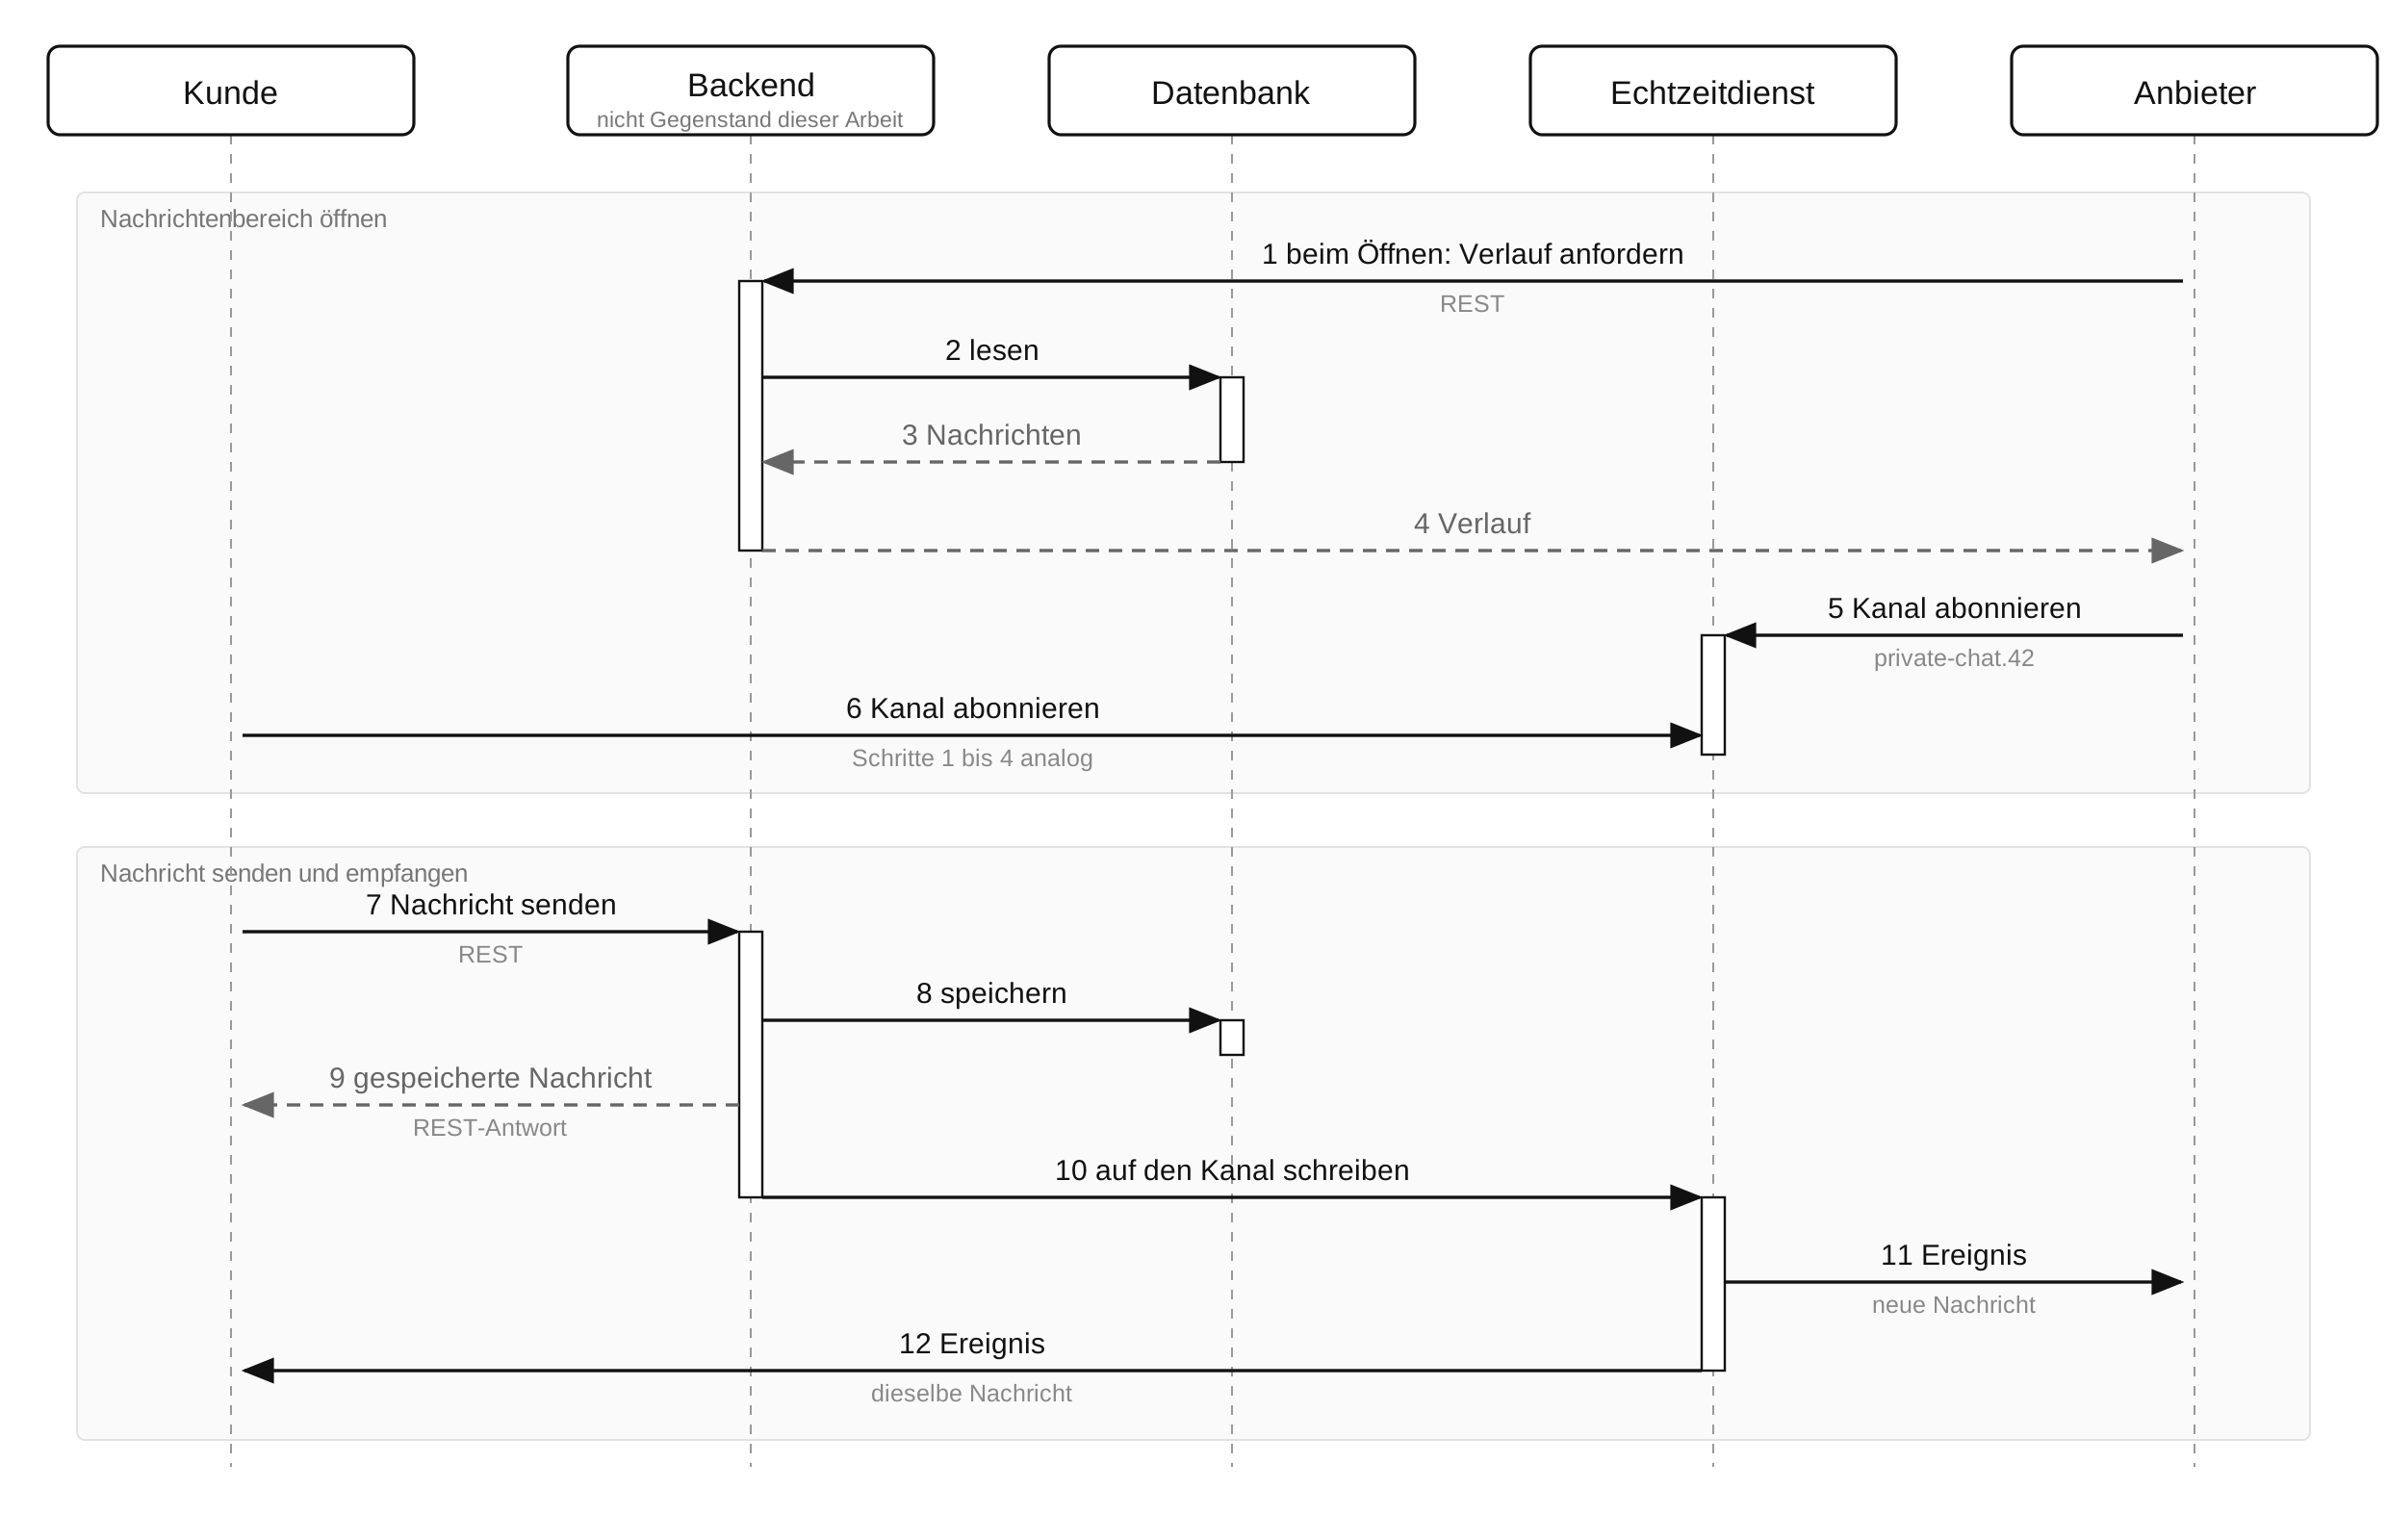
\includegraphics[width=\textwidth]{Bilder/abb_messaging.png}
\caption{Weg einer Nachricht zwischen Absender und Empfänger
(eigene Darstellung)}
\label{fig:messaging_ablauf}
\end{figure}
 
Neben der Unterhaltung selbst ist eine zweite Angabe in Echtzeit zu
übertragen: die Anzahl ungelesener Nachrichten. Sie wird in der
Kopfzeile angezeigt und muss sich auch dann aktualisieren, wenn der
Nutzer sich an einer beliebigen anderen Stelle der Anwendung
befindet. Da die Kanäle der Unterhaltungen dort nicht abonniert
sind, erhält jeder Nutzer zusätzlich einen auf ihn bezogenen Kanal,
über den ausschließlich dieser Zählerstand übermittelt wird.
 
Schließlich sieht der Entwurf drei Zustände je Nachricht vor:
gesendet, zugestellt und gelesen. Der Absender erkennt daran, ob
seine Nachricht angekommen ist und ob der Empfänger sie gelesen hat
(vgl. Abschnitt~\ref{subsec:gestaltungsprinzipien}).